\section{Frames as Basic Display Entities}
When we introduced viewers in \ref{ch:task} and \ref{sec:viewers},
we simplified the abstraction aim.
We know already that viewers appear as elements of 2nd order in the tiling hierarchy.
Having treated them as black boxes so far
we have not revealed anything about the hierarchy continuation.
As a matter of fact, viewers are neither elementary display entities nor atoms.
They are just a special case of so-called \emph{(display) frames}.
They are arbitrary rectangles displaying a collection of objects or a document excerpt.
In particular, they may recursively contain other frames, a capability
that makes them an extremely powerful tool for any display organizer.

Type \verb|Frame| is declared as
\begin{verbatim}
  Frame = POINTER TO FrameDesc;
  FrameDesc = RECORD next, dsc: Frame;
                    X, Y, W, H: INT;
                        handle: Handler END;
\end{verbatim}
\verb|next| and \verb|dsc| are connections to further frames,
whose names suggest a recursive hierarchical structure:
\begin{table}[h!]
  \centering
  \begin{tabular}{r l}
           & points to \\\hline
    $next$ & the next frame on the same level, while \\
    $dsc$  & the (1st) descendant, i.e. the next lower \\
           & level of the nested frames hierarchy.
  \end{tabular}
\end{table}
\\\verb|X|, \verb|Y|, \verb|W|, \verb|H|, and the handler \verb|handle| serve the original purpose
to which we introduced them. In particular, the handler allows frames to react individually
on the receipt of messages:
\begin{verbatim}
  Handler = PROC(F: Frame; VAR M: FrameMsg);
\end{verbatim}
where \verb|FrameMsg| represents the root of a potentially unlimited tree hierarchy
of possible messages to frames:
\begin{verbatim}
  FrameMsg = RECORD END;
\end{verbatim}
Having now introduced the concept of frames, we can reveal the whole truth about viewers.
As a matter of fact, \verb|Viewer| is a derived type, a extension of \verb|Frame|:
\begin{verbatim}
  Viewer = POINTER TO ViewerDesc;
  ViewerDesc = RECORD (FrameDesc) state: INT END;
\end{verbatim}
These declarations formally express the fact that viewers are nothing but a special case
(or variant or subclass) of general frames, additionally featuring a \verb|state| of visibility.
In particular, viewers inherit the hierarchical structure of frames.  This is
an extremely useful property immediately opening an unlimited spectrum of possibilities
for designers of a specific subclass of viewers to organize the representing rectangular area.
For example, the area of viewers of, say, class \verb|Desktop| may take the role of a background
being covered by an arbitrary collection of possibly mutually overlapping frames. In other words,
our decision of using a tiling viewer scheme globally can easily be overwritten locally.

An even more important example of a predefined structure
is provided by the abstract class, called \emph{menu viewers},
whose shape is familiar from most snapshots taken of the standard Oberon display screen.
A menu viewer consists of a thin rectangular boundary line and an interior area
being vertically decomposed into a menu region at the top
and a contents region at the bottom (see Fig \ref{fig:menu}).
\begin{figure}[h!]
  \centering
  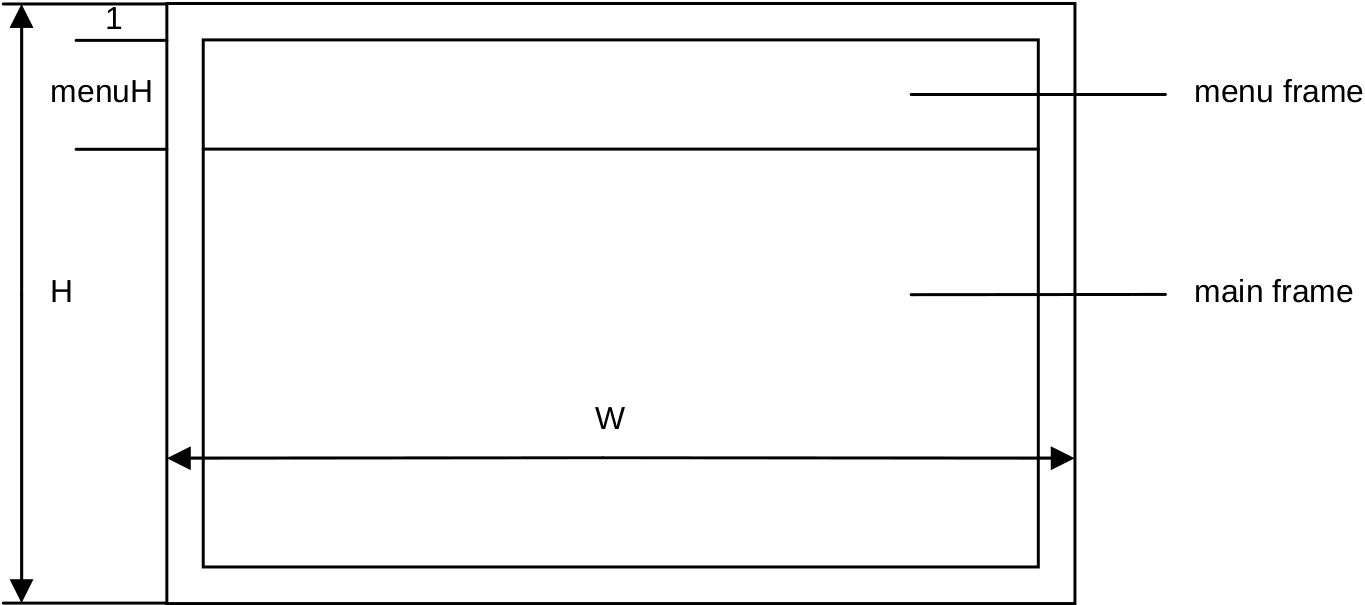
\includegraphics[width=\textwidth]{i/7}
  \caption{The compositional structure of a menu viewer}
  \label{fig:menu}
\end{figure}

In terms of data structures, the class of menu viewers is defined as a type extension of
\verb|Viewer| with an additional component \verb|menuH| specifying the menu frame height:
\begin{verbatim}
  MenuViewer = POINTER TO MenuViewerDesc;
  MenuViewerDesc = RECORD (ViewerDesc) menuH: INT END;
\end{verbatim}
Each menu viewer \verb|V| specifies exactly 2 descendants:
\begin{itemize}
  \item the menu frame \verb|V.dsc|, and
  \item the frame of main contents or main frame \verb|V.dsc.next|.
\end{itemize}
Absolutely nothing is fixed about the 2 descendant frames contents.
The standard menu frame is a text frame, displaying a line of commands in inverse video mode.
By definition, the nature of the main frame specifies its type:
\begin{itemize}
  \item If it is a text frame, we call the viewer a text one;
  \item If a graphics frame, we call it a graphics viewer, etc.
\end{itemize}
